\documentclass[10pt,twocolumn,letterpaper]{article}

\usepackage{cvpr}
\usepackage{times}
\usepackage{epsfig}
\usepackage{graphicx}
\usepackage{amsmath}
\usepackage{amssymb}

\usepackage{subcaption}
\captionsetup{compatibility=false}

% Include other packages here, before hyperref.

% If you comment hyperref and then uncomment it, you should delete
% egpaper.aux before re-running latex.  (Or just hit 'q' on the first latex
% run, let it finish, and you should be clear).
\usepackage[pagebackref=true,breaklinks=true,letterpaper=true,colorlinks,bookmarks=false]{hyperref}

%\cvprfinalcopy % *** Uncomment this line for the final submission

\def\cvprPaperID{Occular Tension} % *** Enter the CVPR Paper ID here
\def\httilde{\mbox{\tt\raisebox{-.5ex}{\symbol{126}}}}

% Pages are numbered in submission mode, and unnumbered in camera-ready
\ifcvprfinal\pagestyle{empty}\fi
\begin{document}

%%%%%%%%% TITLE
\title{Title goes here}

\author{Sajan Patel\\
University of Michigan\\
%Institution1 address\\
{\tt\small sajanptl@umich.edu}
% For a paper whose authors are all at the same institution,
% omit the following lines up until the closing ``}''.
% Additional authors and addresses can be added with ``\and'',
% just like the second author.
% To save space, use either the email address or home page, not both
\and
Shurjo Banerjee\\
University of Michigan\\
%Institution2\\
%First line of institution2 address\\
{\tt\small shurjo@umich.edu}
}

\maketitle
%\thispagestyle{empty}

%%%%%%%%% ABSTRACT
\begin{abstract}
The overall problem of Visual Simultaneous Localization and Mapping (VSLAM) and its different aspects have 
been researched in the computer vision community extensively. This paper critiques three papers on VSLAM 
and provides an analysis of the innovative contributions of each. Robust Large Scale Monocular Simultaneous Localization and Mapping proposes a framework for implementing VSLAM using monocular cameras. SLAM++: Simultaneous Localisation and Mapping at the Level of Objects proposes a method for VLSAM using prior knowledge of the environment and object recognition. Good Features to Track for Visual SLAM (GF-SLAM) focuses on the aspect of finding good visual features to use in VSLAM based on their temporal observability. This paper also provides an analysis of the implementation of the GF-SLAM paper and the recreation of the paper's key experiment.
\end{abstract}

%%%%%%%%% BODY TEXT
\section{Introduction}
The problem of estimating a 3D model the environment as sensed by a camera as well as estimating the 
camera's trajectory is Visual Simultaneous Localization and Mapping (VSLAM).  The computer vision community has researched 
and provided innovative solutions that focus on different aspects of the overall problem. In this paper, we analyze the following three CVPR conference papers on VSLAM, discussing their innovative solution to a particular aspect of VLSAM or the problem as a whole, implementation, and subsequent conclusions: 
1) Robust Large Scale Monocular Visual SLAM [1], 
2) SLAM++: Simultaneous Localisation and Mapping at the Level of Objects [2], and 
3) Good Features to Track for Visual SLAM [3]. We also provide an in-depth analysis of our implementation of Zhang \etal [3] and the conclusions drawn from the reproduction of the paper's key experiment.

%------------------------------------------------------------------------
% Critique of Monocular VSLAM
%-------------------------------------------------------------------------
\section{Robust Large Scale Monocular Visual SLAM}

\subsection{Problem Statement}

The paper focuses on the problem of using calibrated monocular cameras to perform VSLAM while making the 
algorithm robust, accurate, and scalable.  Monocular VSLAM comes with the challenge of not being able to 
observe the scale of the scene of the environment.  In order to overcome this, loop closures 
(which occur when the camera returns to a previously observed location) need to be detected.  
This is an issue in large environments where many scenes look alike, and results in an erroneous 
3D model if loop closures are not detected properly.  Thus, the paper focuses not only on the general 
problem of monocular VSLAM but also tackles 
a key subproblem of dealing with loop closure.

%-------------------------------------------------------------------------
\subsection{Innovative Contribution}

To solve the problem of monocular VSLAM, the authors propose a framework consisting of three parts:
1) a Structure from Motion (SfM) algorithm based on the \textit{Known Rotation Problem} [?]  
is used to estimate submaps which are parts of the camera trajectory and the unknown environment [?],
2) a loopy belief propagation algorithm is used to efficiently aligns many submaps based 
on a graph of relative 3D similarities to produce a global map that is consistent up to a scale factor, and
3) an outlier removal algorithm that detects and removes outliers in the relative 3D similarity 
graph is used to reject wrong loop closures.

\subsection{Proposed Method}
The paper proposes a four-part framework to implement the innovations that solve monocular VSLAM: 
keyframe selection, submap reconstruction, pairwise similarity estimation, and large scale 
relative similarity averaging.

\textbf{Keyframe selection:} For each frame in the captured video, Harris Points of Interest 
(PoI) are detected and tracked using a Lucas-Kanade tracker.  When the Euclidean distance between 
the PoI of the current frame and previously selected keyframe is greater than a specified threshold, the 
frame is selected as a keyframe.

\textbf{Submap reconstruction:} Consecutive keyframes are clustered, and using the 
\textit{Known Rotation Problem}, a SfM algorithm is applied to each one by first extracting the SURF 
PoI [?] from all member keyframes. Loops are closed inside of each submap by 
matching these PoI between pairs of keyframes. The epipolar geometry is then calculated 
using the 5-point algorithm with RANSAC and bundle adjustment [?] between consecutive pairs of images 
using the SURF matches and tracked Harris PoI. The local 3D orientations are then extracted are used to 
estimate the global 3D orientation. With this, known tracks of PoI are built and 
a linear program is used to solve the \textit{Known Rotation Problem} to estimate the camera pose at each 
keyframe and the associated 3D point to reconstruct the submap [?].

\textbf{Pairwise Similarity Estimation:} Loop closures in the reconstructed submaps are 
detected by first applying a bag of words approach on the SURF descriptors of the 3D 
points of all submaps to give each submap a unique descriptor.  After that, the relative 
3D similarities between each keyframe and its 10 nearest nieghboors is estimated by 
matching SURF descriptors with the 3D points of each submap using a k-d tree, 
and then using the 3-points algorithm with RANSAC and nonlinear refinement on 
those matches.

\textbf{Large Scale Similarity Averaging:} To align the submaps by 
estimating thier global 3D similarity to the global reference frame, a cost function on relative 
similarities is minimized by transforming the problem to a graph inference problem.  
Outliers in the graphs (representing wrong loop closures) are rejected by the 
\textit{outlier removal algorithm} in which loop closures are incrementally checked 
by finding the shorted loop of inliers and adding them to the overall graph of inliers 
if their cycle error and covariance are within specified bounds.  
Once the outliers are removed, the \textit{loopy belief propagation algorithm} performs the 
graph inference by accumulating the measurements and variances on temporal 
subgraphs of the original graph as it builds up final average global similarity. 
This algorithm is parallelized, so it can be applied on a large scale of submaps.

\subsection{Experimental Evaluation}
To evaluate the proposed VSLAM framework, the authors compared its performance 
with that of state of the art algorithms [?] and [?] on the TUM and KITTI datasets and 
with four different cameras with different resolutions on indoor videos they captured.  
Each experiment used the same optimized parameters for the various parts of the algorithm.  
When evaluating the results of the algorithms with respect to ground truth, a 3D similarity 
obtained from the minimum distance between the estimated and actual camera trajectories 
was used.  When compared to the [?] on the TUM RGB-D dataset, the author's approach resulted in a 
lower RMSE for camera trajectories than [?].  When compared to [?] on the KITTI dataset, 
the author's algorithm estimated camera trajectories that were closer to ground truth and 
thus performed better. When compared to [?] on their own videos, the proposed 
method outperformed [?] with respect to the ground truth motion of the camera.  
In addition, the paper discusses the limitations of the framework in not being able to 
estimate a pure rotation of the camera, the necessity for the sensed environment 
to be static, and the necessary for consecutive relative similarities to be outlier free. 
However, the framework still has reasonable performance when applied to datasets 
that involve some moving objects.

\subsection{Subsequent Conclusions}
The performance evaluation of the method shows that the authors' proposed monocular VSLAM framework does
 substantiate their claim.  Robust, independent submap generation is achieved by the visual odometry approach 
based on the \textit{Known Rotation Problem}, and these submaps can be processed and aligned to form the 
global map and camera trajectory estimates with loop closure through the outlier removal and loopy belief 
propagation algorithms.  Even with the described limitations, the evaluations show the innovative framework does 
provide a robust, accurate, and scalable solution to loop closure and the overall problem monocular VSLAM.

\section {SLAM++: Simultaneous Localisation and Mapping at the Level of Objects}
\subsection{Problem Statement}
The authors of this paper propose an approach to the VSLAM problem using a combination of the KinectFusion algorithm along with an efficient graph based 3D object recognition system. According to them, this approach offers several advantages over existing VSLAM systems in operation that operate at the level of low level primitives (i.e. points, lines, etc). 

%-------------------------------------------------------------------------
\subsection{Innovative Contribution}
The VSLAM problem has been approached from the perspective of 3D object recognition before. However these methods generally reveal  huge amounts of wasted computational effort via repeated low level geometry processing of the 3D objects. To counter this, the authors propose the building of pose graph maps based on an ``object-oriented" approach that directly encodes the positions of recognized 3D structures. With each new measurement, the graph is continually optimized with new measurements from the sensors and allows for efficient tracking of the camera system based on recognized landmarks. In addition to this, the algorithms make the assumption that the world has ``intrinsic symmetry in the form of repetitive objects" thereby allowing for the the objects in a scene to be identified and segmented as salient repeated elements. The algorithm leverages this repetetiveness along with the efficient use of GPU architectures to provide a real time processing system. 

%-------------------------------------------------------------------------
\subsection{Proposed Method}
\textbf{Creating an Object Database:} The authors first create a database of repeatedly occurring objects via known KinectFusion algorithms. These are objects that are subsequently recognized and used in their VSLAM process. 

\textbf{SLAM Map Representation:} The authors represent the world via a graph where each node stores the 6DOF pose of discovered objects relative to a fixed world frame as well as an annotation of the type of the object from the earlier created database. 

\textbf{Real-Time Object Recognition:} This portion of the method recognizes objects in the world based on standard mesh recognition algorithms. The implementation is parallelized on GPUs to allow the real-time detection of multiple instances of multiple objects. These correspondences are obtained via the use of Point-Pair Features (PPFs) which are four dimensional descriptors. 

\textbf{Camera Tracking and Object Pose Estimation:} The iterative closest point (ICP) algorithm is used to to track the pose of the camera model based on the earlier computed object based locations. A Huber penalty function is used to in this optimization process. Criteria is developed to ensure successful convergence of the tracking error.

\textbf{Graph Optimization:} The poses of the static object is now viewed as a graph optimization problem which minimizes the sum over all the measurement constraints based on the known features of each object.

\textbf{Relocalization:} The system accounts for a loss in camera tracking by re-initilazing localization based on matching at least 3 of the objects seen in the previously tracked long-term graph. 

%-------------------------------------------------------------------------
\subsection{Experimental Evaluation}
The authors reference a video submitted along with this paper to CVPR as a better description of the advantages of their method. 

\textbf{Loop Closure:} Small loop closures are detected and compensated for by the ICP algorithm. Larger loop closures are compensated for via the use of the relocalization method. 

\textbf{Large Scale Mapping:} Scaled mapping of a large room (15mX10mX3m) was obtained along with the mapping of 34 different objects around the room. The algorithm uses no priors regarding the original placement of these objects.

\textbf{Moved Object Detection:} The algorithm also displays the ability to track these objects while they, themselves are in motion. 

\textbf{System Statistics:} The algorithm displays the amount of storage used as compared to the more traditional KinectFusion algorithm. The given mapped rooms is stored in about 20MB of space as compared to the 1.4GB used by KinectFusion. The resultant compression ratio is 1/70 which is a dramatic improvement. 

%-------------------------------------------------------------------------
\subsection{Subsequent Conclusions}
The paper makes several bold claims with regard to its own contributions to the literature. The graph based optimization method does indeed seem novel and the system has significantly large data compression ratio when compared to the KinectFusion algorithm. UnfortunatelyThe experimentally evaluated conclusions are quite sparse when compared to the dense and well written introduction and methodology. The biggest issue pertains from the fact that no standard metric is used to compare the system's advantages and efficiently to other 3D object recognition based VSLAM approaches. Thus, though several claims are made about the paper's VSLAM advantages over other methods, there are no easy ways to determine the validity of these claims.


\section {Good Features to Track for Visual SLAM}

\subsection{Problem Statement}

This paper focuses on the problem of feature selection for VSLAM since not all features 
detected and tracked by conventional methods contribute to the accurate estimation of 
camera trajectories and the overall map.  Only a subset of all tracked and detected features 
actually produces a good result for VSLAM, and furthermore, there are many different ways of
detecting these features. As VSLAM applications grow to include large-scale reconstruction from 
on large sets of features, an efficient algorithm that can be applied to features generated by any 
detection method is necessary. Thus, this paper focuses on finding the best features out of any given 
set of previously detected features as a preprocessing step before VSLAM occurs.

In exploring different methods for VSLAM proposed in recent conference papers, 
we chose to re-implement the methods and key experiment of this paper.

\subsection{Innovative Contribution}
To solve the problem of finding the best features to use for VSLAM given a set of detected features, 
this paper proposes a new SVD-based algorithm for more rigorous feature selection to be used 
during the localization process. The paper develops a mechanism by which such measured features 
can be ranked with an observability score. The ranked feature set can then be used to generate a 
reduced feature set with better a better estimation accuracy. The authors call their system the Good 
Features algorithm (GF-SLAM for short). The innovative contribution of this paper is in the three main 
aspects of GF-SLAM: 1) the system observability measure for features, 2) the rank-k temporal update 
of observability scores, and 3) a submodular learning method for completing the set of good features if 
the initial ranking of scores fails to provide the desired quantity of good features for a given application of 
VSLAM.

\textbf{System Observability Measure}: To counter the use of extraneous features in the localization process 
of a VSLAM system, the paper develops a metric of observability scores based on the temporal observability 
for each detected feature in each captured video frame. Features are represented by their coordinates in the 
image plane as well as the corresponding world coordinates, allowing this measure to be applied to features 
extracted from video frames by any detection method. The general idea is that features with higher temporal 
observability are scored higher and the set of ``good features" is created from all features whose scores are 
above a specified threshold based on the application of VSLAM. These good features are then called 
anchors.

\textbf{Rank-k Temporal Update of Observability Score}: The generation of feature observability 
scores requires 
the computation and storage of large observability matrices that increase over time. 
The actual act of creating these matrices is inefficient and can lead to delays 
in the SLAM process. To counter this, the authors propose a new algorithm to generate the 
observability matrix 
based on an incremental SVD of the system's observability matrix applied per time step.

\textbf{Submodular Learning for Feature Grouping}: The ranking and thresholding of feature 
observability scores may not 
always produce an adequate number of anchors. 
Thus, this paper proposes a submodular learning algorithm that 
greedily chooses the best of the remaining features with scores 
below the threshold to complete the anchor set based on an 
SVD of the augmented system observability matrix of the anchor set and possible upgraded features. 

\subsection{Proposed Method}
\textbf{Dynamical Measurement Model of VSLAM System:}
The authors use a constant velocity motion model that describes the motion of a VSLAM system in standard 
euclidian three space, 
$SE(3)$, as the basis for their algorithm. The method requires the position, and orientation as well as the linear 
and angular velocities 
of the camera model of the VSLAM system: 
\begin{equation} \label{eq:stateVector}
\boldsymbol{x}_{R_k}^W = (\boldsymbol{r}_{R_k}^W \ \ \ \  \boldsymbol{q}_{R_k}^W  \ \ \ \  \boldsymbol{v}_{R_k}^W  \ \ \ \  \boldsymbol{\omega}_{R_k}^W)^T
\end{equation}
where $\boldsymbol{x}_{R_k}^W$ is the state vector of the camera model, 
$\boldsymbol{r}_{R_k}^W$ is its position, 
$\boldsymbol{v}_{R_k}^W$ is its velocity, 
and $\boldsymbol{\omega}_{R_k}^W$ is its angular velocity. All these quantities are with reference to the world frame as denoted by the superscript $W$ at time $k$. 
The state vector is updated with each time segment by the SLAM system. 

The algorithm requires access to the following properties of the features that are located by the SLAM system: 
\begin{equation} \label{eq:featureProjection}
\boldsymbol{p}_{i}^{R_k} = ({p}_{x_i}^{R_k} \ \ \ \  {p}_{y_i}^{R_k}  \ \ \ \  {p}_{z_i}^{R_k})^T
\end{equation}
\begin{equation} \label{eq:featureProjection2}
\boldsymbol{h}_{i}^{R_k} = \begin{bmatrix} {h}_{x_i} \\ {h}_{y_i} \end{bmatrix} = distort(\begin{bmatrix} . \end{bmatrix})
\end{equation}
where $\boldsymbol{p}_{i}^{R_k}$ is the pinhole projection of the features in homogenous coordinates, and 
$\boldsymbol{h}_{x_i}$ is the projection of these coordinates on to the pinhole plane in two dimensions. 
These coordinates are obtained after correcting for distortion which involves the intrinsic parameters of the
 camera.

\textbf{Computation of System Observability Measure:} To compute the observability score for each feature,
the authors define a System Observability Matrix (SOM), ${Q}_{SOM}$. ${Q}_{SOM}$ is defined for a fixed number 
of frames, $\tau$, of the SLAM process. When the current frame iteration grows larger than $\tau$, the oldest
 elements of the now fixed size ${Q}_{SOM}$ are replaced directly by the newest feature values. $\tau$ is 
 thus an important input parameter to the system as it governs the efficiency of the overall algorithm. 
 ${Q}_{SOM}$ itself is built as a function of the current frame number, $j$, where 
 $j<\tau$. 
\begin{equation} \label{eq:qsom}
\boldsymbol{Q}_{SOM}(j) = \begin{bmatrix} \ \ Q_1^T \ | \ Q_2^T \ | \ ... \ | \ Q_j^T  \ \ \end{bmatrix}
\end{equation}

The replacement process for when $j>\tau$ is described in a later section. Each $Q_j^T$ is built and appended to ${Q}_{SOM}$ as the frame number increments. Each $Q_j^T$ itself has the following form: 
\begin{equation} \label{eq:Qjjj}
Q_j^T = \begin{bmatrix} \ \ H_j^T \ | \ (H_j F_j)^T \ | \ ... \ | \ (H_j F_j^{n-1})^T  \ \ \end{bmatrix}
\end{equation}
where $F$ is the process matrix that relates the motion model defined in \eqref{eq:stateVector} 
from one state to the next. $H$ is the measurement Jacobian where the derivatives are arranged as follows (with features and anchors abbreviated as ``feat." and ``anch." respectively):

\noindent{}$\begin{bmatrix}
\small{\text{image feat. w.r.t. camera state}}&\small{\text{image feat. w.r.t. world feat.}}\\
\small{\text{image anch. w.r.t. camera state}}&0
\end{bmatrix}$\\


Once $Q_{SOM}$ is computed, the temporal observability scores for each feature is computed as:
\begin{equation} \label{eq:Qjjj}
score(f) = \sigma_{min}(Q_{SOM} \ for \ feature \ f)
\end{equation}

\textbf{Rank-k Temporal Update of Observability Score:} As can be seen from the preceding section, the computation of $Q_{SOM}$ is an extensive operation. To simplify matters the authors present an iterated SVD approach to creating $Q_{SOM}$ when $j>3$  and $j<\tau + 1$ . 

Fundamentally, $Q_{SOM}$ is created via \eqref{eq:qsom} 
for the first three frames. For subsequent frames, the SVD of $Q_{SOM}$ and combined with corresponding calculated ${Q}_{j}$ in \eqref{eq:Qjjj} to form the new $Q_{SOM}$ . Again, this new definitions of several matrices and involves diagonalization of newly constructed matrices. Please refer to the original text for the complete implementation details. The net gain by the algorithm is the creation of $Q_{SOM}$ by a rank-2r update instead of creating a whole new matrix. 

For $j>\tau + 1$ , $Q_{SOM}$ is updated via replacement. The newest ${Q}_{j}$ in \eqref{eq:Qjjj} is computed and placed in the positions occupied by the oldest elements of the matrix. As an example, if at time k, $Q_{SOM}(k) = \begin{bmatrix} \ \ Q_1^T \ | \ Q_2^T \ | \ ... \ | \ Q_k^T  \ \ \end{bmatrix}$, then at time k+1, the oldest (i.e. the first element) is replaced, ${Q}_{SOM}(k+1) = \begin{bmatrix}\ \ Q_{k+1}^T \ | \ Q_2^T \ | \ ... \ | \ Q_k^T\ \ \end{bmatrix}$.

\textbf{Submodular Learning for Feature Grouping:} If the set of anchors created after the thresholding of the feature observability scores is smaller than desired, a greedy submodular learning algorithm upgrades features with with the next best scores to anchors to complete the anchor set. This is done by creating an SOM of just the anchors and candidate rows for each remaining feature. The algorithm iterates through each candidate feature, appending it's row to the end of the anchor SOM and then taking the SVD of that matrix to get the observability score for that feature via \eqref{eq:Qjjj} with the modification that $Q_{SOM}$ is now the anchor and candidate row SOM. The feature whose row produces the maximum observability score is upgraded to be an anchor and removed from the set of features. This greedy algorithm recomputes the anchor and candidate SOMs and repeats the process until the the desired number of anchors is obtained.

\begin{figure*}[t!]
        \begin{subfigure}[b]{0.25\textwidth}
                \fbox{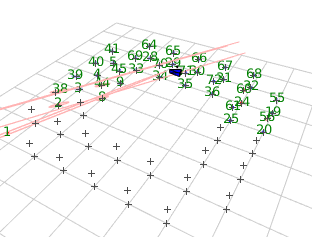
\includegraphics[height = 3.5cm, width=\linewidth]{Figures/AllFeatures_SLAM.png}}
                \caption{VSLAM (all features)}
                \label{fig:gull}
        \end{subfigure}%
        \begin{subfigure}[b]{0.25\textwidth}
                \fbox{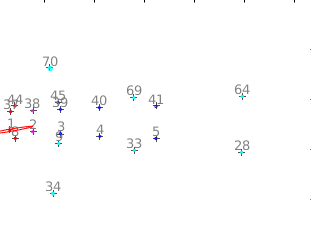
\includegraphics[height = 3.5cm, width=\linewidth]{Figures/AllFeatures_Pinhole.png}}
                \caption{Pinhole View (all features)}
                \label{fig:gull2}
        \end{subfigure}%  
        \begin{subfigure}[b]{0.25\textwidth}
                \fbox{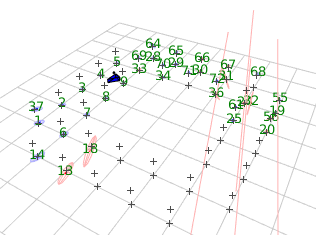
\includegraphics[height = 3.5cm, width=\linewidth]{Figures/FewerFeatures_SLAM.png}}
                \caption{VSLAM (10 ranked feat.)}
                \label{fig:tiger}
        \end{subfigure}%
        \begin{subfigure}[b]{0.25\textwidth}
                \fbox{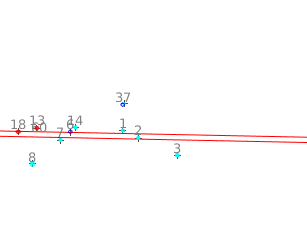
\includegraphics[height = 3.5cm, width=\linewidth]{Figures/FewerFeatures_Pinhole.png}}
                \caption{Pinhole View (10 ranked feat.)}
                \label{fig:mouse}
        \end{subfigure}
        \caption{Experimental Results: (a) VSLAM is performed using all the features. All the landmarks (+ signs) are detected by the robot and used for localization. (b) Shows the pinhole view of the robot in the first scene. These pixel coordinates form the $\boldsymbol{h}_{x_i}$ that \eqref{eq:featureProjection2} used in the algorithm. (c) VSLAM is performed with the the 10 highest ranked features. In the figure this is apparent from the fact that all the landmarks in the vicinity of the robot are not labelled. (d) Corresponding pinhole view. As expected, fewer features are being used for the localization process.}
\label{fig:animals}
\end{figure*}

\subsection{Experimental Method}
The authors implemented their feature reduction algorithm on readily 
available simulated VSLAM data that was created by the authors of 
%%%%%%%%%
[31]. 
%%%%%%%%%%%%%%%%%%%%%%
The robot is made to move in a circular in a simulated environment of dimensions 12mX12m with 72 
landmarks forming a square. The VSLAM process uses an Extended Kalman Filter to estimate the locations 
of each landmark and subsequent estimate its own position in the map. In the original EKF algorithm, the 
simulated robot detects as many landmarks that it can detect. The authors apply their SVD ranking approach
 to select a certain subset of the number of features selected. By changing the number of features used as 
 well as the observation noise, they run the VSLAM simulation several times and compare their results to 
 that of the original algorithm. They run each simulation 40 times and count the number of times their 
 algorithm outperforms the original. The noise values used are $\sigma=\{0.5, 1.0, 1.5, 2.0, 2.5\} $. 
The number of features used are $ K = \{ 3, 4, 5, 6, 7, 8, 10, 12 \}$. 
The results are provided in Table 1. 
\begin{table}[h]
\begin{center}
\begin{tabular}{|c|c|c|}
\hline
Metric Used & Num. Succesful & Accuracy  \\
\hline
 Translation Error &   &   \\
$ \sum_k || \Delta \boldsymbol{r}_{R_k}^W ||_2 $ & 37/40 & 92.5\% \\ 
%&   &   \\
\hline
Rotation Error &   &   \\
$ \sum_k || \Delta \boldsymbol{\theta}_{R_k}^W ||_2 $ & 33/40 & 82.5\% \\
%&   & \\
\hline
\end{tabular}
\end{center}
\caption{Author's experimental results.}
\end{table}

\subsection{Our Implementation}
We chose to re-implement this ranked features algorithm. The first step was to download and run the original VSLAM EKF algorithm [31] that was used by the authors in their experimentation. The code was readily available to download and use online on the author's page.

\textbf{Algorithm Structure:} The algorithm simulates a robot moving in a circular trajectory surrounded by 72 detectable landmarks. A monocular camera is placed on the robot for visual sensing purposes. Broadly the algorithm is divided in to the following sections:
\begin{enumerate}
  \item Data Generation - The trajectory to be followed by the robot is generated. Each landmarks's position is also generated. Care is taken to seed the random number generator at a fixed point so as to ensure consistency across measurements.
  \item Simulation - The simulated robot is moved ahead on the predefined trajectory. The measurement vectors are generated based on the location of the landmarks located by the robot. In the terms of our implementation, we consider the features to be these landmark positions. 
 \item Localization - The robot's current position and orientation is localized by sending all the detected features to an Extended Kalman Filtering Algorithm.
\item Visualization - The corresponding position of the landmarks, detected features, actual robot's position and orientation and estimated robot's position and orientation are visually updated on a three dimensional plot.
\end{enumerate}

\textbf{Calculating $\boldsymbol{Q}_{SOM}$:} The first step to generating the observability matrix was to map the features detected by the SLAM algorithm to their corresponding $\boldsymbol{p}_{i}^{R_k}$'s \eqref{eq:featureProjection} and $\boldsymbol{h}_{x_i}$ \eqref{eq:featureProjection2} indices.This is done between step 2 and 3 by extracting the corresponding elements from the algorithms pinhole perspective calculations. The camera's corresponding position and orientation, $\boldsymbol{x}_{R_k}^W$ \eqref{eq:stateVector} , is also extracted. These features are now used to create a corresponding $H$ matrix which in turn is used to iteratively build up $Q_{SOM}$ as described in \eqref{eq:qsom} and \eqref{eq:Qjjj} . $Q_{SOM}$ is created to contain information from 10 iterations of the EKF algorithm at a time i.e. $\tau = 10$ . As described previously, $Q_{SOM}$ is initially created iteratively, then via the iterative SVD and finally via the replacement method.
  
\textbf{Feature Scoring:} Step two provides us with a list of features that has been detected by the robot. Each of these features have corresponding rows in the $Q_{SOM}$ matrix. For each feature, the corresponding rows are iteratively extracted and concatenated to form a feature matrix. 
The SVD is computed for each of these matrices and the minimum positive singular value is extracted as a
 corresponding score of each feature by \eqref{eq:qsom}. 
 The resultant scores are then used to sort the original features as well 
as the corresponding $\boldsymbol{p}_{i}^{R_k}$'s \eqref{eq:featureProjection} and $\boldsymbol{h}_{x_i}$'s 
\eqref{eq:featureProjection2}. A subset of the scored features with scores above an 
application-specified threshold is designated as the anchor set and is passed on to the localization step and the algorithm proceeds as normal.

\textbf{Submodular Learning:} We implemented submodular learning to complete the anchor set as described by the paper's proposed greedy algorithm. This portion of the implementation also runs only if the resultant set of anchors after thresholding the feature scores is less than 2 below the desired number of anchors.

\textbf{Experimental Implementation:} The experiment described by the authors is recreated exactly. 40 experiments are performed at a fixed seeded location. The experiment is run over 200 iterations for each combination of pixel noise and number of anchors from the follow sets: $\sigma=\{0.5, 1.0, 1.5, 2.0, 2.5\} $ and $ K = \{ 3, 4, 5, 6, 7, 8, 10, 12 \}$. The positional and euclidian 2-norms are used to compare the results of the original algorithm vs. the ranked features method.

\textbf{Experimental Results:} Table 2 results obtained in terms of the positional norm. 
Table 3 provides the results obtained in terms of the Euclidian norm. 
???The ranked algorithm performed better then the original in 8/40 cases (20\%) 
in terms of the positional norm. In terms of the euclidian norm it performed better 14/40 cases (35\%). For a complete tabulation of all the results please refer to the attached appendix.
\begin{table}[h]
\begin{center}
\begin{tabular}{|c|c|c|}
\hline
$\sigma$ & Avg. ($ \sum_k || \Delta \boldsymbol{r}_{R_k}^W ||_2)_{all} $ & Avg. ($ \sum_k || \Delta \boldsymbol{r}_{R_k}^W ||_2)_{rnk} $ \\
\hline
0.5  & 6.3591  &  7.0524\\
\hline
1.0  &  4.8382 &  8.9654\\
\hline
1.5  &  6.1305 &  10.1870\\
\hline
2.0  &  6.5744 &  7.0839\\
\hline
2.5  &  6.4082 &  8.5952\\
\hline
\end{tabular}
\end{center}
\caption{Position Based Results}
\end{table}

\begin{table}[t]
\begin{center}
\begin{tabular}{|c|c|c|}
\hline
$\sigma$ & Avg. ($ \sum_k || \Delta \boldsymbol{\theta}_{R_k}^W ||_2)_{all} $ & Avg. ($ \sum_k || \Delta \boldsymbol{\theta}_{R_k}^W ||_2)_{rnk} $  \\
\hline
0.5  & 0.7082  &  7.2744 \\
\hline
1.0  &  0.9237 &  5.8175 \\
\hline
1.5  &  0.8389 &  8.5750 \\
\hline
2.0  &  7.9474 &  4.7680 \\
\hline
2.5  &  8.0217 &  6.1176 \\
\hline
\end{tabular}
\end{center}
\caption{Euclidian Norm Based Results}
\end{table}

\subsection{Subsequent Conclusions}
As can be seen, the results we obtained do not agree with that of the authors' though the experiment is reproduced exactly. We believe the reason for this an incorrect creation of the $Q_{SOM}$ matrix. This paper turned out to be particularly difficult to re-implement. The main reason behind this was the convoluted mathematical definitions and notations used by the authors especially with regard to the contents and creation of $Q_{SOM}$. We tried to contact the authors via email but are unfortunately yet to hear back from them. They also do not provide any of the software or code used.

In conclusion, based on the metric they define, the author's feature ranking algorithm appears to successfully aid SLAM processes. Unfortunately, their results do not appear to be easy to reproduce. For this algorithm to achieve more success in the community it is our suggestion that the authors clean up their mathematical notation as well as release commented software and code which performs the algorithm successfully.    

\section{Conclusion}

Conclusion goes here.

%\section{Introduction}
%
%Please follow the steps outlined below when submitting your manuscript to
%the IEEE Computer Society Press.  This style guide now has several
%important modifications (for example, you are no longer warned against the
%use of sticky tape to attach your artwork to the paper), so all authors
%should read this new version.
%
%%-------------------------------------------------------------------------
%\subsection{Language}
%
%All manuscripts must be in English.
%
%\subsection{Dual submission}
%
%Please refer to the author guidelines on the CVPR 2016 web page for a
%discussion of the policy on dual submissions.
%
%\subsection{Paper length}
%Papers, excluding the references section,
%must be no longer than eight pages in length. The references section
%will not be included in the page count, and there is no limit on the
%length of the references section. For example, a paper of eight pages
%with two pages of references would have a total length of 10 pages.
%{\bf There will be no extra page charges for CVPR 2016.}
%
%Overlength papers will simply not be reviewed.  This includes papers
%where the margins and formatting are deemed to have been significantly
%altered from those laid down by this style guide.  Note that this
%\LaTeX\ guide already sets figure captions and references in a smaller font.
%The reason such papers will not be reviewed is that there is no provision for
%supervised revisions of manuscripts.  The reviewing process cannot determine
%the suitability of the paper for presentation in eight pages if it is
%reviewed in eleven.  
%
%%-------------------------------------------------------------------------
%\subsection{The ruler}
%The \LaTeX\ style defines a printed ruler which should be present in the
%version submitted for review.  The ruler is provided in order that
%reviewers may comment on particular lines in the paper without
%circumlocution.  If you are preparing a document using a non-\LaTeX\
%document preparation system, please arrange for an equivalent ruler to
%appear on the final output pages.  The presence or absence of the ruler
%should not change the appearance of any other content on the page.  The
%camera ready copy should not contain a ruler. (\LaTeX\ users may uncomment
%the \verb'\cvprfinalcopy' command in the document preamble.)  Reviewers:
%note that the ruler measurements do not align well with lines in the paper
%--- this turns out to be very difficult to do well when the paper contains
%many figures and equations, and, when done, looks ugly.  Just use fractional
%references (e.g.\ this line is $095.5$), although in most cases one would
%expect that the approximate location will be adequate.
%
%\subsection{Mathematics}
%
%Please number all of your sections and displayed equations.  It is
%important for readers to be able to refer to any particular equation.  Just
%because you didn't refer to it in the text doesn't mean some future reader
%might not need to refer to it.  It is cumbersome to have to use
%circumlocutions like ``the equation second from the top of page 3 column
%1''.  (Note that the ruler will not be present in the final copy, so is not
%an alternative to equation numbers).  All authors will benefit from reading
%Mermin's description of how to write mathematics:
%\url{http://www.pamitc.org/documents/mermin.pdf}.
%
%
%\subsection{Blind review}
%
%Many authors misunderstand the concept of anonymizing for blind
%review.  Blind review does not mean that one must remove
%citations to one's own work---in fact it is often impossible to
%review a paper unless the previous citations are known and
%available.
%
%Blind review means that you do not use the words ``my'' or ``our''
%when citing previous work.  That is all.  (But see below for
%techreports.)
%
%Saying ``this builds on the work of Lucy Smith [1]'' does not say
%that you are Lucy Smith; it says that you are building on her
%work.  If you are Smith and Jones, do not say ``as we show in
%[7]'', say ``as Smith and Jones show in [7]'' and at the end of the
%paper, include reference 7 as you would any other cited work.
%
%An example of a bad paper just asking to be rejected:
%\begin{quote}
%\begin{center}
%    An analysis of the frobnicatable foo filter.
%\end{center}
%
%   In this paper we present a performance analysis of our
%   previous paper [1], and show it to be inferior to all
%   previously known methods.  Why the previous paper was
%   accepted without this analysis is beyond me.
%
%   [1] Removed for blind review
%\end{quote}
%
%
%An example of an acceptable paper:
%
%\begin{quote}
%\begin{center}
%     An analysis of the frobnicatable foo filter.
%\end{center}
%
%   In this paper we present a performance analysis of the
%   paper of Smith \etal [1], and show it to be inferior to
%   all previously known methods.  Why the previous paper
%   was accepted without this analysis is beyond me.
%
%   [1] Smith, L and Jones, C. ``The frobnicatable foo
%   filter, a fundamental contribution to human knowledge''.
%   Nature 381(12), 1-213.
%\end{quote}
%
%If you are making a submission to another conference at the same time,
%which covers similar or overlapping material, you may need to refer to that
%submission in order to explain the differences, just as you would if you
%had previously published related work.  In such cases, include the
%anonymized parallel submission~\cite{Authors14} as additional material and
%cite it as
%\begin{quote}
%[1] Authors. ``The frobnicatable foo filter'', F\&G 2014 Submission ID 324,
%Supplied as additional material {\tt fg324.pdf}.
%\end{quote}
%
%Finally, you may feel you need to tell the reader that more details can be
%found elsewhere, and refer them to a technical report.  For conference
%submissions, the paper must stand on its own, and not {\em require} the
%reviewer to go to a techreport for further details.  Thus, you may say in
%the body of the paper ``further details may be found
%in~\cite{Authors14b}''.  Then submit the techreport as additional material.
%Again, you may not assume the reviewers will read this material.
%
%Sometimes your paper is about a problem which you tested using a tool which
%is widely known to be restricted to a single institution.  For example,
%let's say it's 1969, you have solved a key problem on the Apollo lander,
%and you believe that the CVPR70 audience would like to hear about your
%solution.  The work is a development of your celebrated 1968 paper entitled
%``Zero-g frobnication: How being the only people in the world with access to
%the Apollo lander source code makes us a wow at parties'', by Zeus \etal.
%
%You can handle this paper like any other.  Don't write ``We show how to
%improve our previous work [Anonymous, 1968].  This time we tested the
%algorithm on a lunar lander [name of lander removed for blind review]''.
%That would be silly, and would immediately identify the authors. Instead
%write the following:
%\begin{quotation}
%\noindent
%   We describe a system for zero-g frobnication.  This
%   system is new because it handles the following cases:
%   A, B.  Previous systems [Zeus et al. 1968] didn't
%   handle case B properly.  Ours handles it by including
%   a foo term in the bar integral.
%
%   ...
%
%   The proposed system was integrated with the Apollo
%   lunar lander, and went all the way to the moon, don't
%   you know.  It displayed the following behaviours
%   which show how well we solved cases A and B: ...
%\end{quotation}
%As you can see, the above text follows standard scientific convention,
%reads better than the first version, and does not explicitly name you as
%the authors.  A reviewer might think it likely that the new paper was
%written by Zeus \etal, but cannot make any decision based on that guess.
%He or she would have to be sure that no other authors could have been
%contracted to solve problem B.
%
%FAQ: Are acknowledgements OK?  No.  Leave them for the final copy.
%
%
%\begin{figure}[t]
%\begin{center}
%\fbox{\rule{0pt}{2in} \rule{0.9\linewidth}{0pt}}
%   %\includegraphics[width=0.8\linewidth]{egfigure.eps}
%\end{center}
%   \caption{Example of caption.  It is set in Roman so that mathematics
%   (always set in Roman: $B \sin A = A \sin B$) may be included without an
%   ugly clash.}
%\label{fig:long}
%\label{fig:onecol}
%\end{figure}
%
%\subsection{Miscellaneous}
%
%\noindent
%Compare the following:\\
%\begin{tabular}{ll}
% \verb'$conf_a$' &  $conf_a$ \\
% \verb'$\mathit{conf}_a$' & $\mathit{conf}_a$
%\end{tabular}\\
%See The \TeX book, p165.
%
%The space after \eg, meaning ``for example'', should not be a
%sentence-ending space. So \eg is correct, {\em e.g.} is not.  The provided
%\verb'\eg' macro takes care of this.
%
%When citing a multi-author paper, you may save space by using ``et alia'',
%shortened to ``\etal'' (not ``{\em et.\ al.}'' as ``{\em et}'' is a complete word.)
%However, use it only when there are three or more authors.  Thus, the
%following is correct: ``
%   Frobnication has been trendy lately.
%   It was introduced by Alpher~\cite{Alpher02}, and subsequently developed by
%   Alpher and Fotheringham-Smythe~\cite{Alpher03}, and Alpher \etal~\cite{Alpher04}.''
%
%This is incorrect: ``... subsequently developed by Alpher \etal~\cite{Alpher03} ...''
%because reference~\cite{Alpher03} has just two authors.  If you use the
%\verb'\etal' macro provided, then you need not worry about double periods
%when used at the end of a sentence as in Alpher \etal.
%
%For this citation style, keep multiple citations in numerical (not
%chronological) order, so prefer \cite{Alpher03,Alpher02,Authors14} to
%\cite{Alpher02,Alpher03,Authors14}.
%
%
%\begin{figure*}
%\begin{center}
%\fbox{\rule{0pt}{2in} \rule{.9\linewidth}{0pt}}
%\end{center}
%   \caption{Example of a short caption, which should be centered.}
%\label{fig:short}
%\end{figure*}
%
%%------------------------------------------------------------------------
%\section{Formatting your paper}
%
%All text must be in a two-column format. The total allowable width of the
%text area is $6\frac78$ inches (17.5 cm) wide by $8\frac78$ inches (22.54
%cm) high. Columns are to be $3\frac14$ inches (8.25 cm) wide, with a
%$\frac{5}{16}$ inch (0.8 cm) space between them. The main title (on the
%first page) should begin 1.0 inch (2.54 cm) from the top edge of the
%page. The second and following pages should begin 1.0 inch (2.54 cm) from
%the top edge. On all pages, the bottom margin should be 1-1/8 inches (2.86
%cm) from the bottom edge of the page for $8.5 \times 11$-inch paper; for A4
%paper, approximately 1-5/8 inches (4.13 cm) from the bottom edge of the
%page.
%
%%-------------------------------------------------------------------------
%\subsection{Margins and page numbering}
%
%All printed material, including text, illustrations, and charts, must be kept
%within a print area 6-7/8 inches (17.5 cm) wide by 8-7/8 inches (22.54 cm)
%high.
%
%
%
%%-------------------------------------------------------------------------
%\subsection{Type-style and fonts}
%
%Wherever Times is specified, Times Roman may also be used. If neither is
%available on your word processor, please use the font closest in
%appearance to Times to which you have access.
%
%MAIN TITLE. Center the title 1-3/8 inches (3.49 cm) from the top edge of
%the first page. The title should be in Times 14-point, boldface type.
%Capitalize the first letter of nouns, pronouns, verbs, adjectives, and
%adverbs; do not capitalize articles, coordinate conjunctions, or
%prepositions (unless the title begins with such a word). Leave two blank
%lines after the title.
%
%AUTHOR NAME(s) and AFFILIATION(s) are to be centered beneath the title
%and printed in Times 12-point, non-boldface type. This information is to
%be followed by two blank lines.
%
%The ABSTRACT and MAIN TEXT are to be in a two-column format.
%
%MAIN TEXT. Type main text in 10-point Times, single-spaced. Do NOT use
%double-spacing. All paragraphs should be indented 1 pica (approx. 1/6
%inch or 0.422 cm). Make sure your text is fully justified---that is,
%flush left and flush right. Please do not place any additional blank
%lines between paragraphs.
%
%Figure and table captions should be 9-point Roman type as in
%Figures~\ref{fig:onecol} and~\ref{fig:short}.  Short captions should be centred.
%
%\noindent Callouts should be 9-point Helvetica, non-boldface type.
%Initially capitalize only the first word of section titles and first-,
%second-, and third-order headings.
%
%FIRST-ORDER HEADINGS. (For example, {\large \bf 1. Introduction})
%should be Times 12-point boldface, initially capitalized, flush left,
%with one blank line before, and one blank line after.
%
%SECOND-ORDER HEADINGS. (For example, { \bf 1.1. Database elements})
%should be Times 11-point boldface, initially capitalized, flush left,
%with one blank line before, and one after. If you require a third-order
%heading (we discourage it), use 10-point Times, boldface, initially
%capitalized, flush left, preceded by one blank line, followed by a period
%and your text on the same line.
%
%%-------------------------------------------------------------------------
%\subsection{Footnotes}
%
%Please use footnotes\footnote {This is what a footnote looks like.  It
%often distracts the reader from the main flow of the argument.} sparingly.
%Indeed, try to avoid footnotes altogether and include necessary peripheral
%observations in
%the text (within parentheses, if you prefer, as in this sentence).  If you
%wish to use a footnote, place it at the bottom of the column on the page on
%which it is referenced. Use Times 8-point type, single-spaced.
%
%
%%-------------------------------------------------------------------------
%\subsection{References}
%
%List and number all bibliographical references in 9-point Times,
%single-spaced, at the end of your paper. When referenced in the text,
%enclose the citation number in square brackets, for
%example~\cite{Authors14}.  Where appropriate, include the name(s) of
%editors of referenced books.
%
%\begin{table}
%\begin{center}
%\begin{tabular}{|l|c|}
%\hline
%Method & Frobnability \\
%\hline\hline
%Theirs & Frumpy \\
%Yours & Frobbly \\
%Ours & Makes one's heart Frob\\
%\hline
%\end{tabular}
%\end{center}
%\caption{Results.   Ours is better.}
%\end{table}
%
%%-------------------------------------------------------------------------
%\subsection{Illustrations, graphs, and photographs}
%
%All graphics should be centered.  Please ensure that any point you wish to
%make is resolvable in a printed copy of the paper.  Resize fonts in figures
%to match the font in the body text, and choose line widths which render
%effectively in print.  Many readers (and reviewers), even of an electronic
%copy, will choose to print your paper in order to read it.  You cannot
%insist that they do otherwise, and therefore must not assume that they can
%zoom in to see tiny details on a graphic.
%
%When placing figures in \LaTeX, it's almost always best to use
%\verb+\includegraphics+, and to specify the  figure width as a multiple of
%the line width as in the example below
%{\small\begin{verbatim}
%   \usepackage[dvips]{graphicx} ...
%   \includegraphics[width=0.8\linewidth]
%                   {myfile.eps}
%\end{verbatim}
%}
%
%
%%-------------------------------------------------------------------------
%\subsection{Color}
%
%Please refer to the author guidelines on the CVPR 2016 web page for a discussion
%of the use of color in your document.
%
%%------------------------------------------------------------------------
%\section{Final copy}
%
%You must include your signed IEEE copyright release form when you submit
%your finished paper. We MUST have this form before your paper can be
%published in the proceedings.
%
%Please direct any questions to the production editor in charge of these
%proceedings at the IEEE Computer Society Press: Phone (714) 821-8380, or
%Fax (714) 761-1784.

{\small
\bibliographystyle{ieee}
%\bibliography{egbib}
}



\end{document}
